% Options for packages loaded elsewhere
\PassOptionsToPackage{unicode}{hyperref}
\PassOptionsToPackage{hyphens}{url}
%
\documentclass[
  doc]{apa6}
\usepackage{amsmath,amssymb}
\usepackage{iftex}
\ifPDFTeX
  \usepackage[T1]{fontenc}
  \usepackage[utf8]{inputenc}
  \usepackage{textcomp} % provide euro and other symbols
\else % if luatex or xetex
  \usepackage{unicode-math} % this also loads fontspec
  \defaultfontfeatures{Scale=MatchLowercase}
  \defaultfontfeatures[\rmfamily]{Ligatures=TeX,Scale=1}
\fi
\usepackage{lmodern}
\ifPDFTeX\else
  % xetex/luatex font selection
\fi
% Use upquote if available, for straight quotes in verbatim environments
\IfFileExists{upquote.sty}{\usepackage{upquote}}{}
\IfFileExists{microtype.sty}{% use microtype if available
  \usepackage[]{microtype}
  \UseMicrotypeSet[protrusion]{basicmath} % disable protrusion for tt fonts
}{}
\makeatletter
\@ifundefined{KOMAClassName}{% if non-KOMA class
  \IfFileExists{parskip.sty}{%
    \usepackage{parskip}
  }{% else
    \setlength{\parindent}{0pt}
    \setlength{\parskip}{6pt plus 2pt minus 1pt}}
}{% if KOMA class
  \KOMAoptions{parskip=half}}
\makeatother
\usepackage{xcolor}
\usepackage{color}
\usepackage{fancyvrb}
\newcommand{\VerbBar}{|}
\newcommand{\VERB}{\Verb[commandchars=\\\{\}]}
\DefineVerbatimEnvironment{Highlighting}{Verbatim}{commandchars=\\\{\}}
% Add ',fontsize=\small' for more characters per line
\usepackage{framed}
\definecolor{shadecolor}{RGB}{248,248,248}
\newenvironment{Shaded}{\begin{snugshade}}{\end{snugshade}}
\newcommand{\AlertTok}[1]{\textcolor[rgb]{0.94,0.16,0.16}{#1}}
\newcommand{\AnnotationTok}[1]{\textcolor[rgb]{0.56,0.35,0.01}{\textbf{\textit{#1}}}}
\newcommand{\AttributeTok}[1]{\textcolor[rgb]{0.13,0.29,0.53}{#1}}
\newcommand{\BaseNTok}[1]{\textcolor[rgb]{0.00,0.00,0.81}{#1}}
\newcommand{\BuiltInTok}[1]{#1}
\newcommand{\CharTok}[1]{\textcolor[rgb]{0.31,0.60,0.02}{#1}}
\newcommand{\CommentTok}[1]{\textcolor[rgb]{0.56,0.35,0.01}{\textit{#1}}}
\newcommand{\CommentVarTok}[1]{\textcolor[rgb]{0.56,0.35,0.01}{\textbf{\textit{#1}}}}
\newcommand{\ConstantTok}[1]{\textcolor[rgb]{0.56,0.35,0.01}{#1}}
\newcommand{\ControlFlowTok}[1]{\textcolor[rgb]{0.13,0.29,0.53}{\textbf{#1}}}
\newcommand{\DataTypeTok}[1]{\textcolor[rgb]{0.13,0.29,0.53}{#1}}
\newcommand{\DecValTok}[1]{\textcolor[rgb]{0.00,0.00,0.81}{#1}}
\newcommand{\DocumentationTok}[1]{\textcolor[rgb]{0.56,0.35,0.01}{\textbf{\textit{#1}}}}
\newcommand{\ErrorTok}[1]{\textcolor[rgb]{0.64,0.00,0.00}{\textbf{#1}}}
\newcommand{\ExtensionTok}[1]{#1}
\newcommand{\FloatTok}[1]{\textcolor[rgb]{0.00,0.00,0.81}{#1}}
\newcommand{\FunctionTok}[1]{\textcolor[rgb]{0.13,0.29,0.53}{\textbf{#1}}}
\newcommand{\ImportTok}[1]{#1}
\newcommand{\InformationTok}[1]{\textcolor[rgb]{0.56,0.35,0.01}{\textbf{\textit{#1}}}}
\newcommand{\KeywordTok}[1]{\textcolor[rgb]{0.13,0.29,0.53}{\textbf{#1}}}
\newcommand{\NormalTok}[1]{#1}
\newcommand{\OperatorTok}[1]{\textcolor[rgb]{0.81,0.36,0.00}{\textbf{#1}}}
\newcommand{\OtherTok}[1]{\textcolor[rgb]{0.56,0.35,0.01}{#1}}
\newcommand{\PreprocessorTok}[1]{\textcolor[rgb]{0.56,0.35,0.01}{\textit{#1}}}
\newcommand{\RegionMarkerTok}[1]{#1}
\newcommand{\SpecialCharTok}[1]{\textcolor[rgb]{0.81,0.36,0.00}{\textbf{#1}}}
\newcommand{\SpecialStringTok}[1]{\textcolor[rgb]{0.31,0.60,0.02}{#1}}
\newcommand{\StringTok}[1]{\textcolor[rgb]{0.31,0.60,0.02}{#1}}
\newcommand{\VariableTok}[1]{\textcolor[rgb]{0.00,0.00,0.00}{#1}}
\newcommand{\VerbatimStringTok}[1]{\textcolor[rgb]{0.31,0.60,0.02}{#1}}
\newcommand{\WarningTok}[1]{\textcolor[rgb]{0.56,0.35,0.01}{\textbf{\textit{#1}}}}
\usepackage{graphicx}
\makeatletter
\def\maxwidth{\ifdim\Gin@nat@width>\linewidth\linewidth\else\Gin@nat@width\fi}
\def\maxheight{\ifdim\Gin@nat@height>\textheight\textheight\else\Gin@nat@height\fi}
\makeatother
% Scale images if necessary, so that they will not overflow the page
% margins by default, and it is still possible to overwrite the defaults
% using explicit options in \includegraphics[width, height, ...]{}
\setkeys{Gin}{width=\maxwidth,height=\maxheight,keepaspectratio}
% Set default figure placement to htbp
\makeatletter
\def\fps@figure{htbp}
\makeatother
\setlength{\emergencystretch}{3em} % prevent overfull lines
\providecommand{\tightlist}{%
  \setlength{\itemsep}{0pt}\setlength{\parskip}{0pt}}
\setcounter{secnumdepth}{5}
% Make \paragraph and \subparagraph free-standing
\ifx\paragraph\undefined\else
  \let\oldparagraph\paragraph
  \renewcommand{\paragraph}[1]{\oldparagraph{#1}\mbox{}}
\fi
\ifx\subparagraph\undefined\else
  \let\oldsubparagraph\subparagraph
  \renewcommand{\subparagraph}[1]{\oldsubparagraph{#1}\mbox{}}
\fi
\newlength{\cslhangindent}
\setlength{\cslhangindent}{1.5em}
\newlength{\csllabelwidth}
\setlength{\csllabelwidth}{3em}
\newlength{\cslentryspacingunit} % times entry-spacing
\setlength{\cslentryspacingunit}{\parskip}
\newenvironment{CSLReferences}[2] % #1 hanging-ident, #2 entry spacing
 {% don't indent paragraphs
  \setlength{\parindent}{0pt}
  % turn on hanging indent if param 1 is 1
  \ifodd #1
  \let\oldpar\par
  \def\par{\hangindent=\cslhangindent\oldpar}
  \fi
  % set entry spacing
  \setlength{\parskip}{#2\cslentryspacingunit}
 }%
 {}
\usepackage{calc}
\newcommand{\CSLBlock}[1]{#1\hfill\break}
\newcommand{\CSLLeftMargin}[1]{\parbox[t]{\csllabelwidth}{#1}}
\newcommand{\CSLRightInline}[1]{\parbox[t]{\linewidth - \csllabelwidth}{#1}\break}
\newcommand{\CSLIndent}[1]{\hspace{\cslhangindent}#1}
\ifLuaTeX
\usepackage[bidi=basic]{babel}
\else
\usepackage[bidi=default]{babel}
\fi
\babelprovide[main,import]{english}
% get rid of language-specific shorthands (see #6817):
\let\LanguageShortHands\languageshorthands
\def\languageshorthands#1{}
% Manuscript styling
\usepackage{upgreek}
\captionsetup{font=singlespacing,justification=justified}

% Table formatting
\usepackage{longtable}
\usepackage{lscape}
% \usepackage[counterclockwise]{rotating}   % Landscape page setup for large tables
\usepackage{multirow}		% Table styling
\usepackage{tabularx}		% Control Column width
\usepackage[flushleft]{threeparttable}	% Allows for three part tables with a specified notes section
\usepackage{threeparttablex}            % Lets threeparttable work with longtable

% Create new environments so endfloat can handle them
% \newenvironment{ltable}
%   {\begin{landscape}\centering\begin{threeparttable}}
%   {\end{threeparttable}\end{landscape}}
\newenvironment{lltable}{\begin{landscape}\centering\begin{ThreePartTable}}{\end{ThreePartTable}\end{landscape}}

% Enables adjusting longtable caption width to table width
% Solution found at http://golatex.de/longtable-mit-caption-so-breit-wie-die-tabelle-t15767.html
\makeatletter
\newcommand\LastLTentrywidth{1em}
\newlength\longtablewidth
\setlength{\longtablewidth}{1in}
\newcommand{\getlongtablewidth}{\begingroup \ifcsname LT@\roman{LT@tables}\endcsname \global\longtablewidth=0pt \renewcommand{\LT@entry}[2]{\global\advance\longtablewidth by ##2\relax\gdef\LastLTentrywidth{##2}}\@nameuse{LT@\roman{LT@tables}} \fi \endgroup}

% \setlength{\parindent}{0.5in}
% \setlength{\parskip}{0pt plus 0pt minus 0pt}

% Overwrite redefinition of paragraph and subparagraph by the default LaTeX template
% See https://github.com/crsh/papaja/issues/292
\makeatletter
\renewcommand{\paragraph}{\@startsection{paragraph}{4}{\parindent}%
  {0\baselineskip \@plus 0.2ex \@minus 0.2ex}%
  {-1em}%
  {\normalfont\normalsize\bfseries\itshape\typesectitle}}

\renewcommand{\subparagraph}[1]{\@startsection{subparagraph}{5}{1em}%
  {0\baselineskip \@plus 0.2ex \@minus 0.2ex}%
  {-\z@\relax}%
  {\normalfont\normalsize\itshape\hspace{\parindent}{#1}\textit{\addperi}}{\relax}}
\makeatother

\makeatletter
\usepackage{etoolbox}
\patchcmd{\maketitle}
  {\section{\normalfont\normalsize\abstractname}}
  {\section*{\normalfont\normalsize\abstractname}}
  {}{\typeout{Failed to patch abstract.}}
\patchcmd{\maketitle}
  {\section{\protect\normalfont{\@title}}}
  {\section*{\protect\normalfont{\@title}}}
  {}{\typeout{Failed to patch title.}}
\makeatother

\usepackage{xpatch}
\makeatletter
\xapptocmd\appendix
  {\xapptocmd\section
    {\addcontentsline{toc}{section}{\appendixname\ifoneappendix\else~\theappendix\fi\\: #1}}
    {}{\InnerPatchFailed}%
  }
{}{\PatchFailed}
\keywords{papaja, NRW80+, descriptive statistics}
\usepackage{csquotes}
\usepackage[titles]{tocloft}
\cftpagenumbersoff{figure}
\renewcommand{\cftfigpresnum}{\itshape\figurename\enspace}
\renewcommand{\cftfigaftersnum}{.\space}
\setlength{\cftfigindent}{0pt}
\setlength{\cftafterloftitleskip}{0pt}
\settowidth{\cftfignumwidth}{Figure 10.\qquad}
\cftpagenumbersoff{table}
\renewcommand{\cfttabpresnum}{\itshape\tablename\enspace}
\renewcommand{\cfttabaftersnum}{.\space}
\setlength{\cfttabindent}{0pt}
\setlength{\cftafterloftitleskip}{0pt}
\settowidth{\cfttabnumwidth}{Table 10.\qquad}
\ifLuaTeX
  \usepackage{selnolig}  % disable illegal ligatures
\fi
\IfFileExists{bookmark.sty}{\usepackage{bookmark}}{\usepackage{hyperref}}
\IfFileExists{xurl.sty}{\usepackage{xurl}}{} % add URL line breaks if available
\urlstyle{same}
\hypersetup{
  pdftitle={Descriptive Statistics of the NRW80+ Dataset},
  pdfauthor={Prof.~Dr.~Stephan Huber1,2},
  pdflang={en-EN},
  pdfkeywords={papaja, NRW80+, descriptive statistics},
  hidelinks,
  pdfcreator={LaTeX via pandoc}}

\title{Descriptive Statistics of the NRW80+ Dataset}
\author{Prof.~Dr.~Stephan Huber\textsuperscript{1,2}}
\date{}


\shorttitle{Descriptive Statistics of the NRW80+ Dataset}

\authornote{

All files related to that paper are hostes on github. see: \url{https://github.com/hubchev/ewa}.

Correspondence concerning this article should be addressed to Prof.~Dr.~Stephan Huber, Im Mediapark 4e. E-mail: \href{mailto:stephan.huber@hs-fresenius.de}{\nolinkurl{stephan.huber@hs-fresenius.de}}

}

\affiliation{\vspace{0.5cm}\textsuperscript{1} Fresenius University of Applied Science\\\textsuperscript{2} Charlotte Fresenius University}

\abstract{%
In this paper, I illustrate the process of importing NRW80+ data (see Zank, Woopen, Wagner, Rietz, \& Kaspar, 2022) into R. Additionally, I present descriptive statistics and graphical visualizations to gain insights into Likert-scaled surveys. The paper adheres to the APA style, implementing the R template provided by the `papaja' package (Aust \& Barth, 2023).
}



\begin{document}
\maketitle

{
\setcounter{tocdepth}{3}
\tableofcontents
}
\hypertarget{technical-note}{%
\section{Technical Note}\label{technical-note}}

In the following, I load (and install) packages that I use later on and I show information about my R session with \texttt{sessionInfo()}.

\begin{Shaded}
\begin{Highlighting}[]
\CommentTok{\# (Install and) load pacman package }
\ControlFlowTok{if}\NormalTok{ (}\SpecialCharTok{!}\FunctionTok{require}\NormalTok{(pacman)) }\FunctionTok{install.packages}\NormalTok{(}\StringTok{"pacman"}\NormalTok{)}

\CommentTok{\# load packages that are already installed and install packages that are not }
\CommentTok{\# installed yet and then load them:}
\NormalTok{pacman}\SpecialCharTok{::}\FunctionTok{p\_load}\NormalTok{(tinylabels, }
\NormalTok{               papaja,}
\NormalTok{               haven, }
\NormalTok{               labelled, }
\NormalTok{               janitor,}
\NormalTok{               skimr, }
\NormalTok{               rstatix, }
\NormalTok{               HH, }
\NormalTok{               likert, }
\NormalTok{               expss,}
\NormalTok{               tidyr, }
\NormalTok{               ggstats,}
\NormalTok{               psych,}
\NormalTok{               sjlabelled,}
\NormalTok{               sjmisc,}
\NormalTok{               tidyverse, }
\NormalTok{               MASS,}
\NormalTok{               dplyr,}
\NormalTok{               magick)}

\FunctionTok{sessionInfo}\NormalTok{()}
\end{Highlighting}
\end{Shaded}

\begin{verbatim}
## R version 4.3.1 (2023-06-16)
## Platform: x86_64-pc-linux-gnu (64-bit)
## Running under: Debian GNU/Linux 12 (bookworm)
## 
## Matrix products: default
## BLAS:   /usr/lib/x86_64-linux-gnu/blas/libblas.so.3.11.0 
## LAPACK: /usr/lib/x86_64-linux-gnu/lapack/liblapack.so.3.11.0
## 
## locale:
##  [1] LC_CTYPE=en_US.UTF-8       LC_NUMERIC=C               LC_TIME=en_US.UTF-8        LC_COLLATE=en_US.UTF-8    
##  [5] LC_MONETARY=en_US.UTF-8    LC_MESSAGES=en_US.UTF-8    LC_PAPER=en_US.UTF-8       LC_NAME=C                 
##  [9] LC_ADDRESS=C               LC_TELEPHONE=C             LC_MEASUREMENT=en_US.UTF-8 LC_IDENTIFICATION=C       
## 
## time zone: Europe/Berlin
## tzcode source: system (glibc)
## 
## attached base packages:
## [1] grid      stats     graphics  grDevices utils     datasets  methods   base     
## 
## other attached packages:
##  [1] magick_2.8.1        lubridate_1.9.3     forcats_1.0.0       stringr_1.5.1       dplyr_1.1.4        
##  [6] purrr_1.0.2         readr_2.1.4         tibble_3.2.1        tidyverse_2.0.0     sjmisc_2.8.9       
## [11] sjlabelled_1.2.0    psych_2.3.9         ggstats_0.5.1       tidyr_1.3.0         expss_0.11.6       
## [16] maditr_0.8.4        likert_1.3.5        xtable_1.8-4        ggplot2_3.4.4       HH_3.1-49          
## [21] gridExtra_2.3       multcomp_1.4-25     TH.data_1.1-2       MASS_7.3-60         survival_3.5-7     
## [26] mvtnorm_1.2-3       latticeExtra_0.6-30 lattice_0.22-5      rstatix_0.7.2       skimr_2.1.5        
## [31] janitor_2.2.0       labelled_2.12.0     haven_2.5.3         papaja_0.1.2.9000   tinylabels_0.2.4   
## [36] pacman_0.5.1       
## 
## loaded via a namespace (and not attached):
##   [1] sylly_0.1-6               later_1.3.1               splines_4.3.1             datawizard_0.9.0         
##   [5] rpart_4.1.21              lifecycle_1.0.4           insight_0.19.6            vcd_1.4-11               
##   [9] backports_1.4.1           magrittr_2.0.3            Hmisc_5.1-1               rmarkdown_2.25.2         
##  [13] yaml_2.3.7                httpuv_1.6.12             RColorBrewer_1.1-3        abind_1.4-5              
##  [17] pkgload_1.3.3             rvest_1.0.3               nnet_7.3-19               rmdfiltr_0.1.3           
##  [21] sandwich_3.0-2            svglite_2.1.2             codetools_0.2-19          xml2_1.3.5               
##  [25] tidyselect_1.2.0          gmp_0.7-4                 effectsize_0.8.6          matrixStats_1.2.0        
##  [29] base64enc_0.1-3           webshot_0.5.5             jsonlite_1.8.7            Formula_1.2-5            
##  [33] ellipsis_0.3.2            emmeans_1.8.9             systemfonts_1.0.5         tools_4.3.1              
##  [37] Rcpp_1.0.11               glue_1.6.2                mnormt_2.1.1              xfun_0.41                
##  [41] withr_2.5.2               fastmap_1.1.1             fansi_1.0.5               digest_0.6.33            
##  [45] mime_0.12                 timechange_0.2.0          R6_2.5.1                  estimability_1.4.1       
##  [49] colorspace_2.1-0          koRpus_0.13-8             jpeg_0.1-10               utf8_1.2.4               
##  [53] generics_0.1.3            data.table_1.14.8         httr_1.4.7                htmlwidgets_1.6.3        
##  [57] parameters_0.21.3         pkgconfig_2.0.3           gtable_0.3.4              Rmpfr_0.9-5              
##  [61] lmtest_0.9-40             htmltools_0.5.7           carData_3.0-5             bookdown_0.36            
##  [65] scales_1.2.1              leaps_3.1                 png_0.1-8                 snakecase_0.11.1         
##  [69] knitr_1.45                rstudioapi_0.15.0         tzdb_0.4.0                reshape2_1.4.4           
##  [73] coda_0.19-4               checkmate_2.3.0           nlme_3.1-163              repr_1.1.6               
##  [77] zoo_1.8-12                parallel_4.3.1            foreign_0.8-85            pillar_1.9.0             
##  [81] vctrs_0.6.4               promises_1.2.1            car_3.1-2                 cluster_2.1.4            
##  [85] htmlTable_2.4.2           evaluate_0.23             tinytex_0.49              cli_3.6.1                
##  [89] compiler_4.3.1            rlang_1.1.2               interp_1.1-5              plyr_1.8.9               
##  [93] stringi_1.8.2             deldir_2.0-2              viridisLite_0.4.2         assertthat_0.2.1         
##  [97] munsell_0.5.0             bayestestR_0.13.1         Matrix_1.6-3              hms_1.1.3                
## [101] wordcountaddin_0.3.0.9000 shiny_1.8.0               broom_1.0.5
\end{verbatim}

\hypertarget{import-data}{%
\section{Import Data}\label{import-data}}

I host a R script on my GitHub account (see \url{https://raw.githubusercontent.com/hubchev/courses/main/scr/readin_GESIS.R}) that explains how to import the NRW80+ data. I have manually saved the data, \texttt{gesis.RData}, in a subfolder named \texttt{data}.

\hypertarget{how-to-use-the-nrw80-data}{%
\section{How to Use the NRW80+ Data}\label{how-to-use-the-nrw80-data}}

\hypertarget{sec-load}{%
\subsection{Load and Subset Data}\label{sec-load}}

I load the data and select some variables that are of particular interest to me.

\begin{Shaded}
\begin{Highlighting}[]
\FunctionTok{getwd}\NormalTok{()}
\end{Highlighting}
\end{Shaded}

\begin{verbatim}
## [1] "/home/sthu/Dropbox/hsf/courses/ewa/ewa_all/rmd_desc"
\end{verbatim}

\begin{Shaded}
\begin{Highlighting}[]
\FunctionTok{load}\NormalTok{(}\StringTok{"../data/gesis.RData"}\NormalTok{)}
\NormalTok{df }\OtherTok{\textless{}{-}}\NormalTok{ dfdta }\SpecialCharTok{|\textgreater{}}
  \FunctionTok{select}\NormalTok{(}\FunctionTok{starts\_with}\NormalTok{(}\StringTok{"alter"}\NormalTok{), }
\NormalTok{         ALT\_agegroup, }
\NormalTok{         ALT\_sex, }
\NormalTok{         famst1, famst7, }
\NormalTok{         demtectcorr, }
\NormalTok{         kogstat, }
\NormalTok{         final, }
\NormalTok{         geschlecht)}

\CommentTok{\# Remove the common prefix from all variables}
\NormalTok{df }\OtherTok{\textless{}{-}}\NormalTok{ df }\SpecialCharTok{|\textgreater{}} 
  \FunctionTok{mutate\_all}\NormalTok{(}\SpecialCharTok{\textasciitilde{}} \FunctionTok{set\_label}\NormalTok{(., }\FunctionTok{gsub}\NormalTok{(}\StringTok{"\^{}Alternserleben: "}\NormalTok{, }\StringTok{""}\NormalTok{, }\FunctionTok{get\_label}\NormalTok{(.))))}
\end{Highlighting}
\end{Shaded}

For simplification, let us focus on the questions that refer to the ``Experience of Ageing'' and create a new dataset \texttt{df\_alterl} that contains only those questions:

\begin{Shaded}
\begin{Highlighting}[]
\NormalTok{df\_alterl }\OtherTok{\textless{}{-}}\NormalTok{ df }\SpecialCharTok{|\textgreater{}} 
  \FunctionTok{select}\NormalTok{(alterl1, }
\NormalTok{         alterl2, }
\NormalTok{         alterl3, }
\NormalTok{         alterl4, }
\NormalTok{         alterl5, }
\NormalTok{         alterl6, }
\NormalTok{         alterl7, }
\NormalTok{         alterl8, }
\NormalTok{         alterl9, }
\NormalTok{         alterl10) }\SpecialCharTok{|\textgreater{}} 
  \FunctionTok{drop\_unused\_labels}\NormalTok{() }

\CommentTok{\# to remove unused labels you can use drop\_unused\_labels():}
\NormalTok{df\_alterl\_un }\OtherTok{\textless{}{-}}\NormalTok{ df\_alterl }\SpecialCharTok{|\textgreater{}}
  \FunctionTok{drop\_unused\_labels}\NormalTok{()}



\FunctionTok{summary}\NormalTok{(df\_alterl)}
\end{Highlighting}
\end{Shaded}

\begin{verbatim}
##     alterl1          alterl2          alterl3          alterl4          alterl5         alterl6      
##  Min.   :-2.000   Min.   :-2.000   Min.   :-2.000   Min.   :-2.000   Min.   :-2.00   Min.   :-2.000  
##  1st Qu.: 1.000   1st Qu.: 2.000   1st Qu.: 1.000   1st Qu.: 2.000   1st Qu.: 2.00   1st Qu.: 2.000  
##  Median : 3.000   Median : 4.000   Median : 2.000   Median : 3.000   Median : 3.00   Median : 4.000  
##  Mean   : 2.656   Mean   : 3.282   Mean   : 2.349   Mean   : 2.763   Mean   : 2.99   Mean   : 3.405  
##  3rd Qu.: 4.000   3rd Qu.: 4.000   3rd Qu.: 3.000   3rd Qu.: 4.000   3rd Qu.: 4.00   3rd Qu.: 5.000  
##  Max.   : 5.000   Max.   : 5.000   Max.   : 5.000   Max.   : 5.000   Max.   : 5.00   Max.   : 5.000  
##     alterl7          alterl8          alterl9          alterl10     
##  Min.   :-2.000   Min.   :-2.000   Min.   :-2.000   Min.   :-2.000  
##  1st Qu.: 2.000   1st Qu.: 1.000   1st Qu.: 2.000   1st Qu.: 1.000  
##  Median : 3.000   Median : 3.000   Median : 3.000   Median : 2.000  
##  Mean   : 3.237   Mean   : 2.712   Mean   : 2.969   Mean   : 2.305  
##  3rd Qu.: 4.000   3rd Qu.: 4.000   3rd Qu.: 4.000   3rd Qu.: 3.000  
##  Max.   : 5.000   Max.   : 5.000   Max.   : 5.000   Max.   : 5.000
\end{verbatim}

\hypertarget{get-an-overview-by-counting}{%
\subsection{Get an Overview by Counting}\label{get-an-overview-by-counting}}

\hypertarget{table-of-r-base}{%
\subsubsection{\texorpdfstring{\texttt{table()} of R base}{table() of R base}}\label{table-of-r-base}}

With the \texttt{table()} function, you can count how many observations of each unique value a variable contains:

\begin{Shaded}
\begin{Highlighting}[]
\FunctionTok{table}\NormalTok{(df\_alterl}\SpecialCharTok{$}\NormalTok{alterl1)}
\end{Highlighting}
\end{Shaded}

\begin{verbatim}
## 
## Weiß nicht Verweigert  Gar nicht  Ein wenig      Mäßig      Stark Sehr stark 
##         80          6        390        266        451        511        159
\end{verbatim}

To do that for each variable of a dataset is easy using \texttt{\textasciitilde{}}, the pipe operator, and \texttt{map()} of the package \texttt{purrr} (Wickham \& Henry, 2023):

\begin{Shaded}
\begin{Highlighting}[]
\NormalTok{df\_alterl }\SpecialCharTok{|\textgreater{}} 
  \FunctionTok{map}\NormalTok{(}\SpecialCharTok{\textasciitilde{}} \FunctionTok{table}\NormalTok{(.))}
\end{Highlighting}
\end{Shaded}

\begin{verbatim}
## $alterl1
## .
## Weiß nicht Verweigert  Gar nicht  Ein wenig      Mäßig      Stark Sehr stark 
##         80          6        390        266        451        511        159 
## 
## $alterl2
## .
## Weiß nicht Verweigert  Gar nicht  Ein wenig      Mäßig      Stark Sehr stark 
##         36          4        196        245        379        648        355 
## 
## $alterl3
## .
## Weiß nicht Verweigert  Gar nicht  Ein wenig      Mäßig      Stark Sehr stark 
##         20          3        500        577        403        244        116 
## 
## $alterl4
## .
## Weiß nicht Verweigert  Gar nicht  Ein wenig      Mäßig      Stark Sehr stark 
##        122          8        222        260        527        543        181 
## 
## $alterl5
## .
## Weiß nicht Verweigert  Gar nicht  Ein wenig      Mäßig      Stark Sehr stark 
##        101          4        199        211        452        680        216 
## 
## $alterl6
## .
## Weiß nicht Verweigert  Gar nicht  Ein wenig      Mäßig      Stark Sehr stark 
##         19          3        149        324        358        537        473 
## 
## $alterl7
## .
## Weiß nicht Verweigert  Gar nicht  Ein wenig      Mäßig      Stark Sehr stark 
##         20          2        145        362        471        525        338 
## 
## $alterl8
## .
## Weiß nicht Verweigert  Gar nicht  Ein wenig      Mäßig      Stark Sehr stark 
##         20          3        516        350        325        340        309 
## 
## $alterl9
## .
## Weiß nicht Verweigert  Gar nicht  Ein wenig      Mäßig      Stark Sehr stark 
##         83         10        261        228        425        564        292 
## 
## $alterl10
## .
## Weiß nicht Verweigert  Gar nicht  Ein wenig      Mäßig      Stark Sehr stark 
##         44          7        537        433        486        251        105
\end{verbatim}

Using \texttt{proportions()} returns the conditional proportions:

\begin{Shaded}
\begin{Highlighting}[]
\NormalTok{df\_alterl }\SpecialCharTok{|\textgreater{}} 
  \FunctionTok{map}\NormalTok{(}\SpecialCharTok{\textasciitilde{}} \FunctionTok{proportions}\NormalTok{(}\FunctionTok{table}\NormalTok{(.)))}
\end{Highlighting}
\end{Shaded}

\begin{verbatim}
## $alterl1
## .
##  Weiß nicht  Verweigert   Gar nicht   Ein wenig       Mäßig       Stark  Sehr stark 
## 0.042941492 0.003220612 0.209339775 0.142780462 0.242082662 0.274288782 0.085346216 
## 
## $alterl2
## .
##  Weiß nicht  Verweigert   Gar nicht   Ein wenig       Mäßig       Stark  Sehr stark 
## 0.019323671 0.002147075 0.105206656 0.131508320 0.203435319 0.347826087 0.190552872 
## 
## $alterl3
## .
##  Weiß nicht  Verweigert   Gar nicht   Ein wenig       Mäßig       Stark  Sehr stark 
## 0.010735373 0.001610306 0.268384326 0.309715513 0.216317767 0.130971551 0.062265164 
## 
## $alterl4
## .
##  Weiß nicht  Verweigert   Gar nicht   Ein wenig       Mäßig       Stark  Sehr stark 
## 0.065485776 0.004294149 0.119162641 0.139559850 0.282877080 0.291465378 0.097155126 
## 
## $alterl5
## .
##  Weiß nicht  Verweigert   Gar nicht   Ein wenig       Mäßig       Stark  Sehr stark 
## 0.054213634 0.002147075 0.106816962 0.113258186 0.242619431 0.365002684 0.115942029 
## 
## $alterl6
## .
##  Weiß nicht  Verweigert   Gar nicht   Ein wenig       Mäßig       Stark  Sehr stark 
## 0.010198604 0.001610306 0.079978529 0.173913043 0.192163178 0.288244767 0.253891573 
## 
## $alterl7
## .
##  Weiß nicht  Verweigert   Gar nicht   Ein wenig       Mäßig       Stark  Sehr stark 
## 0.010735373 0.001073537 0.077831455 0.194310252 0.252818035 0.281803543 0.181427805 
## 
## $alterl8
## .
##  Weiß nicht  Verweigert   Gar nicht   Ein wenig       Mäßig       Stark  Sehr stark 
## 0.010735373 0.001610306 0.276972625 0.187869028 0.174449812 0.182501342 0.165861514 
## 
## $alterl9
## .
##  Weiß nicht  Verweigert   Gar nicht   Ein wenig       Mäßig       Stark  Sehr stark 
## 0.044551798 0.005367687 0.140096618 0.122383253 0.228126677 0.302737520 0.156736447 
## 
## $alterl10
## .
##  Weiß nicht  Verweigert   Gar nicht   Ein wenig       Mäßig       Stark  Sehr stark 
## 0.023617821 0.003757381 0.288244767 0.232420827 0.260869565 0.134728932 0.056360709
\end{verbatim}

\hypertarget{tabyl-of-janitor}{%
\subsubsection{\texorpdfstring{\texttt{tabyl()} of \texttt{janitor}}{tabyl() of janitor}}\label{tabyl-of-janitor}}

With \texttt{tabyl()} which is part of \texttt{janitor} (Firke, 2023), we can get both nicely:

\begin{Shaded}
\begin{Highlighting}[]
\NormalTok{df\_alterl }\SpecialCharTok{|\textgreater{}} 
  \FunctionTok{tabyl}\NormalTok{(alterl1) }
\end{Highlighting}
\end{Shaded}

\begin{verbatim}
##  alterl1   n     percent
##       -2  80 0.042941492
##       -1   6 0.003220612
##        1 390 0.209339775
##        2 266 0.142780462
##        3 451 0.242082662
##        4 511 0.274288782
##        5 159 0.085346216
\end{verbatim}

\begin{Shaded}
\begin{Highlighting}[]
\NormalTok{df\_alterl }\SpecialCharTok{|\textgreater{}} 
  \FunctionTok{map}\NormalTok{(}\SpecialCharTok{\textasciitilde{}} \FunctionTok{tabyl}\NormalTok{(.))}
\end{Highlighting}
\end{Shaded}

\begin{verbatim}
## $alterl1
##   .   n     percent
##  -2  80 0.042941492
##  -1   6 0.003220612
##   1 390 0.209339775
##   2 266 0.142780462
##   3 451 0.242082662
##   4 511 0.274288782
##   5 159 0.085346216
## 
## $alterl2
##   .   n     percent
##  -2  36 0.019323671
##  -1   4 0.002147075
##   1 196 0.105206656
##   2 245 0.131508320
##   3 379 0.203435319
##   4 648 0.347826087
##   5 355 0.190552872
## 
## $alterl3
##   .   n     percent
##  -2  20 0.010735373
##  -1   3 0.001610306
##   1 500 0.268384326
##   2 577 0.309715513
##   3 403 0.216317767
##   4 244 0.130971551
##   5 116 0.062265164
## 
## $alterl4
##   .   n     percent
##  -2 122 0.065485776
##  -1   8 0.004294149
##   1 222 0.119162641
##   2 260 0.139559850
##   3 527 0.282877080
##   4 543 0.291465378
##   5 181 0.097155126
## 
## $alterl5
##   .   n     percent
##  -2 101 0.054213634
##  -1   4 0.002147075
##   1 199 0.106816962
##   2 211 0.113258186
##   3 452 0.242619431
##   4 680 0.365002684
##   5 216 0.115942029
## 
## $alterl6
##   .   n     percent
##  -2  19 0.010198604
##  -1   3 0.001610306
##   1 149 0.079978529
##   2 324 0.173913043
##   3 358 0.192163178
##   4 537 0.288244767
##   5 473 0.253891573
## 
## $alterl7
##   .   n     percent
##  -2  20 0.010735373
##  -1   2 0.001073537
##   1 145 0.077831455
##   2 362 0.194310252
##   3 471 0.252818035
##   4 525 0.281803543
##   5 338 0.181427805
## 
## $alterl8
##   .   n     percent
##  -2  20 0.010735373
##  -1   3 0.001610306
##   1 516 0.276972625
##   2 350 0.187869028
##   3 325 0.174449812
##   4 340 0.182501342
##   5 309 0.165861514
## 
## $alterl9
##   .   n     percent
##  -2  83 0.044551798
##  -1  10 0.005367687
##   1 261 0.140096618
##   2 228 0.122383253
##   3 425 0.228126677
##   4 564 0.302737520
##   5 292 0.156736447
## 
## $alterl10
##   .   n     percent
##  -2  44 0.023617821
##  -1   7 0.003757381
##   1 537 0.288244767
##   2 433 0.232420827
##   3 486 0.260869565
##   4 251 0.134728932
##   5 105 0.056360709
\end{verbatim}

\hypertarget{frq-of-sjmisc}{%
\subsubsection{\texorpdfstring{\texttt{frq()} of \texttt{sjmisc}}{frq() of sjmisc}}\label{frq-of-sjmisc}}

As the variables \texttt{df\_alterl1} are factors. Thus, we can use the \texttt{sjmisc} package, see Lüdecke (2018) and the cheatsheet of \texttt{sjmisc} \url{http://strengejacke.de/sjmisc-cheatsheet.pdf}. Also worth a reading is \texttt{browseVignettes("sjmisc")}.

For example, we can use \texttt{frq()} for nice frequency tables:

\begin{Shaded}
\begin{Highlighting}[]
\NormalTok{df\_alterl }\SpecialCharTok{|\textgreater{}} 
  \FunctionTok{map}\NormalTok{(}\SpecialCharTok{\textasciitilde{}} \FunctionTok{frq}\NormalTok{(. , }\AttributeTok{show.na =}\NormalTok{ T))}
\end{Highlighting}
\end{Shaded}

\begin{verbatim}
## $alterl1
## Beziehungen und andere Menschen mehr schätzen (x) <numeric> 
## # total N=1863 valid N=1863 mean=2.66 sd=1.61
## 
## Value |      Label |   N | Raw % | Valid % | Cum. %
## ---------------------------------------------------
##    -2 | Weiß nicht |   0 |  0.00 |    0.00 |   0.00
##    -1 | Verweigert |   0 |  0.00 |    0.00 |   0.00
##     1 |  Gar nicht |  80 |  4.29 |    4.29 |   4.29
##     2 |  Ein wenig |   6 |  0.32 |    0.32 |   4.62
##     3 |      Mäßig | 390 | 20.93 |   20.93 |  25.55
##     4 |      Stark | 266 | 14.28 |   14.28 |  39.83
##     5 | Sehr stark | 451 | 24.21 |   24.21 |  64.04
##     6 |       <NA> | 511 | 27.43 |   27.43 |  91.47
##     7 |       <NA> | 159 |  8.53 |    8.53 | 100.00
##  <NA> |       <NA> |   0 |  0.00 |    <NA> |   <NA>
## 
## $alterl2
## Gesundheit mehr Aufmerksamkeit widmen (x) <numeric> 
## # total N=1863 valid N=1863 mean=3.28 sd=1.45
## 
## Value |      Label |   N | Raw % | Valid % | Cum. %
## ---------------------------------------------------
##    -2 | Weiß nicht |   0 |  0.00 |    0.00 |   0.00
##    -1 | Verweigert |   0 |  0.00 |    0.00 |   0.00
##     1 |  Gar nicht |  36 |  1.93 |    1.93 |   1.93
##     2 |  Ein wenig |   4 |  0.21 |    0.21 |   2.15
##     3 |      Mäßig | 196 | 10.52 |   10.52 |  12.67
##     4 |      Stark | 245 | 13.15 |   13.15 |  25.82
##     5 | Sehr stark | 379 | 20.34 |   20.34 |  46.16
##     6 |       <NA> | 648 | 34.78 |   34.78 |  80.94
##     7 |       <NA> | 355 | 19.06 |   19.06 | 100.00
##  <NA> |       <NA> |   0 |  0.00 |    <NA> |   <NA>
## 
## $alterl3
## geistige Leistungsfähigkeit nimmt ab (x) <numeric> 
## # total N=1863 valid N=1863 mean=2.35 sd=1.28
## 
## Value |      Label |   N | Raw % | Valid % | Cum. %
## ---------------------------------------------------
##    -2 | Weiß nicht |   0 |  0.00 |    0.00 |   0.00
##    -1 | Verweigert |   0 |  0.00 |    0.00 |   0.00
##     1 |  Gar nicht |  20 |  1.07 |    1.07 |   1.07
##     2 |  Ein wenig |   3 |  0.16 |    0.16 |   1.23
##     3 |      Mäßig | 500 | 26.84 |   26.84 |  28.07
##     4 |      Stark | 577 | 30.97 |   30.97 |  59.04
##     5 | Sehr stark | 403 | 21.63 |   21.63 |  80.68
##     6 |       <NA> | 244 | 13.10 |   13.10 |  93.77
##     7 |       <NA> | 116 |  6.23 |    6.23 | 100.00
##  <NA> |       <NA> |   0 |  0.00 |    <NA> |   <NA>
## 
## $alterl4
## mehr Erfahrung, um Dinge und Menschen einzuschätzen (x) <numeric> 
## # total N=1863 valid N=1863 mean=2.76 sd=1.72
## 
## Value |      Label |   N | Raw % | Valid % | Cum. %
## ---------------------------------------------------
##    -2 | Weiß nicht |   0 |  0.00 |    0.00 |   0.00
##    -1 | Verweigert |   0 |  0.00 |    0.00 |   0.00
##     1 |  Gar nicht | 122 |  6.55 |    6.55 |   6.55
##     2 |  Ein wenig |   8 |  0.43 |    0.43 |   6.98
##     3 |      Mäßig | 222 | 11.92 |   11.92 |  18.89
##     4 |      Stark | 260 | 13.96 |   13.96 |  32.85
##     5 | Sehr stark | 527 | 28.29 |   28.29 |  61.14
##     6 |       <NA> | 543 | 29.15 |   29.15 |  90.28
##     7 |       <NA> | 181 |  9.72 |    9.72 | 100.00
##  <NA> |       <NA> |   0 |  0.00 |    <NA> |   <NA>
## 
## $alterl5
## besseres Gespür, was wichtig ist (x) <numeric> 
## # total N=1863 valid N=1863 mean=2.99 sd=1.66
## 
## Value |      Label |   N | Raw % | Valid % | Cum. %
## ---------------------------------------------------
##    -2 | Weiß nicht |   0 |  0.00 |    0.00 |   0.00
##    -1 | Verweigert |   0 |  0.00 |    0.00 |   0.00
##     1 |  Gar nicht | 101 |  5.42 |    5.42 |   5.42
##     2 |  Ein wenig |   4 |  0.21 |    0.21 |   5.64
##     3 |      Mäßig | 199 | 10.68 |   10.68 |  16.32
##     4 |      Stark | 211 | 11.33 |   11.33 |  27.64
##     5 | Sehr stark | 452 | 24.26 |   24.26 |  51.91
##     6 |       <NA> | 680 | 36.50 |   36.50 |  88.41
##     7 |       <NA> | 216 | 11.59 |   11.59 | 100.00
##  <NA> |       <NA> |   0 |  0.00 |    <NA> |   <NA>
## 
## $alterl6
## Einschränkung der Aktivitäten (x) <numeric> 
## # total N=1863 valid N=1863 mean=3.40 sd=1.38
## 
## Value |      Label |   N | Raw % | Valid % | Cum. %
## ---------------------------------------------------
##    -2 | Weiß nicht |   0 |  0.00 |    0.00 |   0.00
##    -1 | Verweigert |   0 |  0.00 |    0.00 |   0.00
##     1 |  Gar nicht |  19 |  1.02 |    1.02 |   1.02
##     2 |  Ein wenig |   3 |  0.16 |    0.16 |   1.18
##     3 |      Mäßig | 149 |  8.00 |    8.00 |   9.18
##     4 |      Stark | 324 | 17.39 |   17.39 |  26.57
##     5 | Sehr stark | 358 | 19.22 |   19.22 |  45.79
##     6 |       <NA> | 537 | 28.82 |   28.82 |  74.61
##     7 |       <NA> | 473 | 25.39 |   25.39 | 100.00
##  <NA> |       <NA> |   0 |  0.00 |    <NA> |   <NA>
## 
## $alterl7
## weniger Energie (x) <numeric> 
## # total N=1863 valid N=1863 mean=3.24 sd=1.32
## 
## Value |      Label |   N | Raw % | Valid % | Cum. %
## ---------------------------------------------------
##    -2 | Weiß nicht |   0 |  0.00 |    0.00 |   0.00
##    -1 | Verweigert |   0 |  0.00 |    0.00 |   0.00
##     1 |  Gar nicht |  20 |  1.07 |    1.07 |   1.07
##     2 |  Ein wenig |   2 |  0.11 |    0.11 |   1.18
##     3 |      Mäßig | 145 |  7.78 |    7.78 |   8.96
##     4 |      Stark | 362 | 19.43 |   19.43 |  28.40
##     5 | Sehr stark | 471 | 25.28 |   25.28 |  53.68
##     6 |       <NA> | 525 | 28.18 |   28.18 |  81.86
##     7 |       <NA> | 338 | 18.14 |   18.14 | 100.00
##  <NA> |       <NA> |   0 |  0.00 |    <NA> |   <NA>
## 
## $alterl8
## Abhängigkeit von der Hilfe Anderer (x) <numeric> 
## # total N=1863 valid N=1863 mean=2.71 sd=1.53
## 
## Value |      Label |   N | Raw % | Valid % | Cum. %
## ---------------------------------------------------
##    -2 | Weiß nicht |   0 |  0.00 |    0.00 |   0.00
##    -1 | Verweigert |   0 |  0.00 |    0.00 |   0.00
##     1 |  Gar nicht |  20 |  1.07 |    1.07 |   1.07
##     2 |  Ein wenig |   3 |  0.16 |    0.16 |   1.23
##     3 |      Mäßig | 516 | 27.70 |   27.70 |  28.93
##     4 |      Stark | 350 | 18.79 |   18.79 |  47.72
##     5 | Sehr stark | 325 | 17.44 |   17.44 |  65.16
##     6 |       <NA> | 340 | 18.25 |   18.25 |  83.41
##     7 |       <NA> | 309 | 16.59 |   16.59 | 100.00
##  <NA> |       <NA> |   0 |  0.00 |    <NA> |   <NA>
## 
## $alterl9
## Freiheit, Tage nach eigenem Willen zu verleben (x) <numeric> 
## # total N=1863 valid N=1863 mean=2.97 sd=1.68
## 
## Value |      Label |   N | Raw % | Valid % | Cum. %
## ---------------------------------------------------
##    -2 | Weiß nicht |   0 |  0.00 |    0.00 |   0.00
##    -1 | Verweigert |   0 |  0.00 |    0.00 |   0.00
##     1 |  Gar nicht |  83 |  4.46 |    4.46 |   4.46
##     2 |  Ein wenig |  10 |  0.54 |    0.54 |   4.99
##     3 |      Mäßig | 261 | 14.01 |   14.01 |  19.00
##     4 |      Stark | 228 | 12.24 |   12.24 |  31.24
##     5 | Sehr stark | 425 | 22.81 |   22.81 |  54.05
##     6 |       <NA> | 564 | 30.27 |   30.27 |  84.33
##     7 |       <NA> | 292 | 15.67 |   15.67 | 100.00
##  <NA> |       <NA> |   0 |  0.00 |    <NA> |   <NA>
## 
## $alterl10
## Motivation fällt schwerer (x) <numeric> 
## # total N=1863 valid N=1863 mean=2.31 sd=1.38
## 
## Value |      Label |   N | Raw % | Valid % | Cum. %
## ---------------------------------------------------
##    -2 | Weiß nicht |   0 |  0.00 |    0.00 |   0.00
##    -1 | Verweigert |   0 |  0.00 |    0.00 |   0.00
##     1 |  Gar nicht |  44 |  2.36 |    2.36 |   2.36
##     2 |  Ein wenig |   7 |  0.38 |    0.38 |   2.74
##     3 |      Mäßig | 537 | 28.82 |   28.82 |  31.56
##     4 |      Stark | 433 | 23.24 |   23.24 |  54.80
##     5 | Sehr stark | 486 | 26.09 |   26.09 |  80.89
##     6 |       <NA> | 251 | 13.47 |   13.47 |  94.36
##     7 |       <NA> | 105 |  5.64 |    5.64 | 100.00
##  <NA> |       <NA> |   0 |  0.00 |    <NA> |   <NA>
\end{verbatim}

\hypertarget{first-summary-statistics}{%
\subsection{First Summary Statistics}\label{first-summary-statistics}}

\hypertarget{using-summary-and-get_summary_stats}{%
\subsubsection{\texorpdfstring{Using \texttt{summary()} and \texttt{get\_summary\_stats()}}{Using summary() and get\_summary\_stats()}}\label{using-summary-and-get_summary_stats}}

First, I am interested in the class of the data and some very basic summary statistics.

\begin{Shaded}
\begin{Highlighting}[]
\FunctionTok{summary}\NormalTok{(df)}
\end{Highlighting}
\end{Shaded}

\begin{verbatim}
##     alterl1          alterl2          alterl3          alterl4          alterl5         alterl6      
##  Min.   :-2.000   Min.   :-2.000   Min.   :-2.000   Min.   :-2.000   Min.   :-2.00   Min.   :-2.000  
##  1st Qu.: 1.000   1st Qu.: 2.000   1st Qu.: 1.000   1st Qu.: 2.000   1st Qu.: 2.00   1st Qu.: 2.000  
##  Median : 3.000   Median : 4.000   Median : 2.000   Median : 3.000   Median : 3.00   Median : 4.000  
##  Mean   : 2.656   Mean   : 3.282   Mean   : 2.349   Mean   : 2.763   Mean   : 2.99   Mean   : 3.405  
##  3rd Qu.: 4.000   3rd Qu.: 4.000   3rd Qu.: 3.000   3rd Qu.: 4.000   3rd Qu.: 4.00   3rd Qu.: 5.000  
##  Max.   : 5.000   Max.   : 5.000   Max.   : 5.000   Max.   : 5.000   Max.   : 5.00   Max.   : 5.000  
##                                                                                                      
##     alterl7          alterl8          alterl9          alterl10        alter_int        alter_cont    
##  Min.   :-2.000   Min.   :-2.000   Min.   :-2.000   Min.   :-2.000   Min.   : 80.00   Min.   : 80.11  
##  1st Qu.: 2.000   1st Qu.: 1.000   1st Qu.: 2.000   1st Qu.: 1.000   1st Qu.: 82.00   1st Qu.: 82.99  
##  Median : 3.000   Median : 3.000   Median : 3.000   Median : 2.000   Median : 86.00   Median : 86.59  
##  Mean   : 3.237   Mean   : 2.712   Mean   : 2.969   Mean   : 2.305   Mean   : 86.48   Mean   : 86.98  
##  3rd Qu.: 4.000   3rd Qu.: 4.000   3rd Qu.: 4.000   3rd Qu.: 3.000   3rd Qu.: 90.00   3rd Qu.: 90.56  
##  Max.   : 5.000   Max.   : 5.000   Max.   : 5.000   Max.   : 5.000   Max.   :102.00   Max.   :102.92  
##                                                                      NA's   :6        NA's   :6       
##    alterl_m1       alterl_m2         alterp        ALT_agegroup      ALT_sex          famst1      
##  Min.   :1.000   Min.   :1.000   Min.   :-4.000   Min.   :1.000   Min.   :1.000   Min.   :-1.000  
##  1st Qu.:2.600   1st Qu.:2.200   1st Qu.:-4.000   1st Qu.:1.000   1st Qu.:1.000   1st Qu.: 1.000  
##  Median :3.200   Median :2.800   Median :-4.000   Median :2.000   Median :2.000   Median : 4.000  
##  Mean   :3.168   Mean   :2.877   Mean   : 2.632   Mean   :1.883   Mean   :1.502   Mean   : 2.765  
##  3rd Qu.:3.800   3rd Qu.:3.600   3rd Qu.:-4.000   3rd Qu.:3.000   3rd Qu.:2.000   3rd Qu.: 4.000  
##  Max.   :5.000   Max.   :5.000   Max.   :99.000   Max.   :3.000   Max.   :2.000   Max.   : 5.000  
##  NA's   :16      NA's   :14                                                                       
##      famst7        demtectcorr         kogstat          final         geschlecht   
##  Min.   :-3.000   Min.   :-11.000   Min.   :-4.00   Min.   :81.00   Min.   :1.000  
##  1st Qu.:-3.000   1st Qu.: -1.000   1st Qu.:-4.00   1st Qu.:81.00   1st Qu.:1.000  
##  Median : 0.000   Median :  0.000   Median :-4.00   Median :81.00   Median :2.000  
##  Mean   :-1.179   Mean   : -1.742   Mean   :-3.21   Mean   :81.09   Mean   :1.502  
##  3rd Qu.: 0.000   3rd Qu.:  0.000   3rd Qu.:-4.00   3rd Qu.:81.00   3rd Qu.:2.000  
##  Max.   : 1.000   Max.   :  2.000   Max.   : 7.00   Max.   :82.00   Max.   :2.000  
## 
\end{verbatim}

\begin{Shaded}
\begin{Highlighting}[]
\NormalTok{sumstat\_alter }\OtherTok{\textless{}{-}}\NormalTok{ df }\SpecialCharTok{|\textgreater{}} 
  \FunctionTok{get\_summary\_stats}\NormalTok{(}
\NormalTok{    alterl1, }
\NormalTok{    alterl2, }
\NormalTok{    alterl3, }
\NormalTok{    alterl4, }
\NormalTok{    alterl5, }
\NormalTok{    alterl6, }
\NormalTok{    alterl7, }
\NormalTok{    alterl8, }
\NormalTok{    alterl9, }
\NormalTok{    alterl10,  }
    \AttributeTok{type =} \StringTok{"five\_number"}\NormalTok{)  }
\end{Highlighting}
\end{Shaded}

\begin{verbatim}
## Warning: attributes are not identical across measure variables; they will be dropped
\end{verbatim}

\begin{Shaded}
\begin{Highlighting}[]
\NormalTok{sumstat\_alter}
\end{Highlighting}
\end{Shaded}

\begin{verbatim}
## # A tibble: 10 x 7
##    variable     n   min   max    q1 median    q3
##    <fct>    <dbl> <dbl> <dbl> <dbl>  <dbl> <dbl>
##  1 alterl1   1863    -2     5     1      3     4
##  2 alterl2   1863    -2     5     2      4     4
##  3 alterl3   1863    -2     5     1      2     3
##  4 alterl4   1863    -2     5     2      3     4
##  5 alterl5   1863    -2     5     2      3     4
##  6 alterl6   1863    -2     5     2      4     5
##  7 alterl7   1863    -2     5     2      3     4
##  8 alterl8   1863    -2     5     1      3     4
##  9 alterl9   1863    -2     5     2      3     4
## 10 alterl10  1863    -2     5     1      2     3
\end{verbatim}

\hypertarget{using-psychdescribe}{%
\subsubsection{\texorpdfstring{Using \texttt{psych::describe()}}{Using psych::describe()}}\label{using-psychdescribe}}

A powerful alternative for descriptive summary statistics is provided by the function \texttt{describe()} of the \texttt{psych} package (William Revelle, 2023).

\begin{Shaded}
\begin{Highlighting}[]
\NormalTok{sumstat\_alter\_psych }\OtherTok{\textless{}{-}}\NormalTok{ df }\SpecialCharTok{|\textgreater{}}
  \FunctionTok{select}\NormalTok{(}\FunctionTok{starts\_with}\NormalTok{(}\StringTok{"alterl"}\NormalTok{)) }\SpecialCharTok{|\textgreater{}} 
\NormalTok{  psych}\SpecialCharTok{::}\FunctionTok{describe}\NormalTok{() }\SpecialCharTok{|\textgreater{}} 
  \FunctionTok{as\_tibble}\NormalTok{(}\AttributeTok{rownames=}\StringTok{"Question"}\NormalTok{)  }\SpecialCharTok{|\textgreater{}} 
  \FunctionTok{select}\NormalTok{(}\SpecialCharTok{{-}}\NormalTok{skew, }\SpecialCharTok{{-}}\NormalTok{kurtosis, }\SpecialCharTok{{-}}\NormalTok{range, }\SpecialCharTok{{-}}\NormalTok{vars) }

\NormalTok{sumstat\_alter\_psych}
\end{Highlighting}
\end{Shaded}

\begin{verbatim}
## # A tibble: 12 x 10
##    Question      n  mean    sd median trimmed   mad   min   max     se
##    <chr>     <dbl> <dbl> <dbl>  <dbl>   <dbl> <dbl> <dbl> <dbl>  <dbl>
##  1 alterl1    1863  2.66 1.61     3      2.76 1.48     -2     5 0.0374
##  2 alterl2    1863  3.28 1.45     4      3.43 1.48     -2     5 0.0336
##  3 alterl3    1863  2.35 1.28     2      2.28 1.48     -2     5 0.0296
##  4 alterl4    1863  2.76 1.72     3      2.96 1.48     -2     5 0.0398
##  5 alterl5    1863  2.99 1.66     3      3.20 1.48     -2     5 0.0385
##  6 alterl6    1863  3.40 1.38     4      3.54 1.48     -2     5 0.0321
##  7 alterl7    1863  3.24 1.32     3      3.33 1.48     -2     5 0.0306
##  8 alterl8    1863  2.71 1.53     3      2.68 1.48     -2     5 0.0355
##  9 alterl9    1863  2.97 1.68     3      3.14 1.48     -2     5 0.0389
## 10 alterl10   1863  2.31 1.38     2      2.28 1.48     -2     5 0.0321
## 11 alterl_m1  1847  3.17 0.829    3.2    3.21 0.890     1     5 0.0193
## 12 alterl_m2  1849  2.88 0.958    2.8    2.86 1.04      1     5 0.0223
\end{verbatim}

\hypertarget{using-summarize-and-the-tidyverse}{%
\subsubsection{\texorpdfstring{Using \texttt{summarize()} and the \texttt{tidyverse}}{Using summarize() and the tidyverse}}\label{using-summarize-and-the-tidyverse}}

As you may be aware, the \texttt{tidyverse} package provides powerful and flexible functions such as \texttt{filter}, \texttt{select}, \texttt{group\_by}, and \texttt{summarize}. Here is an example demonstrating how these functions can be utilized to create descriptive statistic tables:

\begin{Shaded}
\begin{Highlighting}[]
\NormalTok{descriptives }\OtherTok{\textless{}{-}}\NormalTok{ dfdta }\SpecialCharTok{|\textgreater{}}  
  \CommentTok{\# filter(alterl1 \textgreater{} 0) |\textgreater{} }
  \FunctionTok{group\_by}\NormalTok{(geschlecht)  }\SpecialCharTok{|\textgreater{}} 
  \FunctionTok{summarize}\NormalTok{(}
    \AttributeTok{Mean =} \FunctionTok{mean}\NormalTok{(alterl1)}
\NormalTok{    , }\AttributeTok{Count =} \FunctionTok{n}\NormalTok{()}
\NormalTok{    , }\AttributeTok{SD =} \FunctionTok{sd}\NormalTok{(alterl1)}
\NormalTok{    , }\AttributeTok{Min =} \FunctionTok{min}\NormalTok{(alterl1)}
\NormalTok{    , }\AttributeTok{Max =} \FunctionTok{max}\NormalTok{(alterl1)}
\NormalTok{  )}

\NormalTok{descriptives}
\end{Highlighting}
\end{Shaded}

\begin{verbatim}
## # A tibble: 2 x 6
##   geschlecht    Mean Count    SD Min             Max           
##   <dbl+lbl>    <dbl> <int> <dbl> <dbl+lbl>       <dbl+lbl>     
## 1 1 [Männlich]  2.71   927  1.50 -2 [Weiß nicht] 5 [Sehr stark]
## 2 2 [Weiblich]  2.60   936  1.72 -2 [Weiß nicht] 5 [Sehr stark]
\end{verbatim}

\hypertarget{make-apa-tables-using-apa_table}{%
\subsection{\texorpdfstring{Make APA Tables using \texttt{apa\_table()}}{Make APA Tables using apa\_table()}}\label{make-apa-tables-using-apa_table}}

The R output shown above might not meet publishable standards as it requires proper formatting, including a table with a caption and adherence to APA rules. To achieve this, the \texttt{apa\_table()} function is recommended, and further details can be found in Aust and Barth (2020, sec. 4.2).

\begin{Shaded}
\begin{Highlighting}[]
\FunctionTok{apa\_table}\NormalTok{(}
\NormalTok{  sumstat\_alter}
\NormalTok{  , }\AttributeTok{caption =} \StringTok{"Summary Statistics: Experience of Ageing."}
\NormalTok{  , }\AttributeTok{note =} \StringTok{"This table contains all variables of \textasciigrave{}alterl*\textasciigrave{}."}
\NormalTok{  , }\AttributeTok{escape =} \ConstantTok{TRUE}
\NormalTok{  )}
\end{Highlighting}
\end{Shaded}

\begin{table}[tbp]

\begin{center}
\begin{threeparttable}

\caption{\label{tab:tabrstatix}Summary Statistics: Experience of Ageing.}

\begin{tabular}{lllllll}
\toprule
variable & \multicolumn{1}{c}{n} & \multicolumn{1}{c}{min} & \multicolumn{1}{c}{max} & \multicolumn{1}{c}{q1} & \multicolumn{1}{c}{median} & \multicolumn{1}{c}{q3}\\
\midrule
alterl1 & 1,863.00 & -2.00 & 5.00 & 1.00 & 3.00 & 4.00\\
alterl2 & 1,863.00 & -2.00 & 5.00 & 2.00 & 4.00 & 4.00\\
alterl3 & 1,863.00 & -2.00 & 5.00 & 1.00 & 2.00 & 3.00\\
alterl4 & 1,863.00 & -2.00 & 5.00 & 2.00 & 3.00 & 4.00\\
alterl5 & 1,863.00 & -2.00 & 5.00 & 2.00 & 3.00 & 4.00\\
alterl6 & 1,863.00 & -2.00 & 5.00 & 2.00 & 4.00 & 5.00\\
alterl7 & 1,863.00 & -2.00 & 5.00 & 2.00 & 3.00 & 4.00\\
alterl8 & 1,863.00 & -2.00 & 5.00 & 1.00 & 3.00 & 4.00\\
alterl9 & 1,863.00 & -2.00 & 5.00 & 2.00 & 3.00 & 4.00\\
alterl10 & 1,863.00 & -2.00 & 5.00 & 1.00 & 2.00 & 3.00\\
\bottomrule
\addlinespace
\end{tabular}

\begin{tablenotes}[para]
\normalsize{\textit{Anmerkungen.} This table contains all variables of `alterl*`.}
\end{tablenotes}

\end{threeparttable}
\end{center}

\end{table}

\begin{Shaded}
\begin{Highlighting}[]
\FunctionTok{apa\_table}\NormalTok{(}
\NormalTok{  sumstat\_alter\_psych}
\NormalTok{  , }\AttributeTok{caption =} \StringTok{"Summary Statistics: Experience of Ageing (psych)"}
\NormalTok{  , }\AttributeTok{note =} \StringTok{"This table contains all variables of \textasciigrave{}alterl*\textasciigrave{}."}
\NormalTok{  , }\AttributeTok{escape =} \ConstantTok{TRUE}
\NormalTok{)}
\end{Highlighting}
\end{Shaded}

\begin{table}[tbp]

\begin{center}
\begin{threeparttable}

\caption{\label{tab:tabsumstatalterpsych}Summary Statistics: Experience of Ageing (psych)}

\begin{tabular}{llllllllll}
\toprule
Question & \multicolumn{1}{c}{n} & \multicolumn{1}{c}{mean} & \multicolumn{1}{c}{sd} & \multicolumn{1}{c}{median} & \multicolumn{1}{c}{trimmed} & \multicolumn{1}{c}{mad} & \multicolumn{1}{c}{min} & \multicolumn{1}{c}{max} & \multicolumn{1}{c}{se}\\
\midrule
alterl1 & 1,863.00 & 2.66 & 1.61 & 3.00 & 2.76 & 1.48 & -2.00 & 5.00 & 0.04\\
alterl2 & 1,863.00 & 3.28 & 1.45 & 4.00 & 3.43 & 1.48 & -2.00 & 5.00 & 0.03\\
alterl3 & 1,863.00 & 2.35 & 1.28 & 2.00 & 2.28 & 1.48 & -2.00 & 5.00 & 0.03\\
alterl4 & 1,863.00 & 2.76 & 1.72 & 3.00 & 2.96 & 1.48 & -2.00 & 5.00 & 0.04\\
alterl5 & 1,863.00 & 2.99 & 1.66 & 3.00 & 3.20 & 1.48 & -2.00 & 5.00 & 0.04\\
alterl6 & 1,863.00 & 3.40 & 1.38 & 4.00 & 3.54 & 1.48 & -2.00 & 5.00 & 0.03\\
alterl7 & 1,863.00 & 3.24 & 1.32 & 3.00 & 3.33 & 1.48 & -2.00 & 5.00 & 0.03\\
alterl8 & 1,863.00 & 2.71 & 1.53 & 3.00 & 2.68 & 1.48 & -2.00 & 5.00 & 0.04\\
alterl9 & 1,863.00 & 2.97 & 1.68 & 3.00 & 3.14 & 1.48 & -2.00 & 5.00 & 0.04\\
alterl10 & 1,863.00 & 2.31 & 1.38 & 2.00 & 2.28 & 1.48 & -2.00 & 5.00 & 0.03\\
alterl\_m1 & 1,847.00 & 3.17 & 0.83 & 3.20 & 3.21 & 0.89 & 1.00 & 5.00 & 0.02\\
alterl\_m2 & 1,849.00 & 2.88 & 0.96 & 2.80 & 2.86 & 1.04 & 1.00 & 5.00 & 0.02\\
\bottomrule
\addlinespace
\end{tabular}

\begin{tablenotes}[para]
\normalsize{\textit{Anmerkungen.} This table contains all variables of `alterl*`.}
\end{tablenotes}

\end{threeparttable}
\end{center}

\end{table}

\begin{Shaded}
\begin{Highlighting}[]
\FunctionTok{apa\_table}\NormalTok{(}
\NormalTok{  descriptives}
\NormalTok{  , }\AttributeTok{caption =} \StringTok{"Experience of Ageing: Valuing Relationships and Other People }
\StringTok{  More (By Gender)"}
\NormalTok{  , }\AttributeTok{escape =} \ConstantTok{TRUE}
\NormalTok{)}
\end{Highlighting}
\end{Shaded}

\begin{table}[tbp]

\begin{center}
\begin{threeparttable}

\caption{\label{tab:tabdescriptives}Experience of Ageing: Valuing Relationships and Other People 
  More (By Gender)}

\begin{tabular}{llllll}
\toprule
geschlecht & \multicolumn{1}{c}{Mean} & \multicolumn{1}{c}{Count} & \multicolumn{1}{c}{SD} & \multicolumn{1}{c}{Min} & \multicolumn{1}{c}{Max}\\
\midrule
1 & 2.71 & 927 & 1.50 & -2 & 5\\
2 & 2.60 & 936 & 1.72 & -2 & 5\\
\bottomrule
\end{tabular}

\end{threeparttable}
\end{center}

\end{table}

Table \ref{tab:tabrstatix} was created with the function \texttt{get\_summary\_stats()} of the \texttt{rstatix} package (Kassambara, 2023), Tables \ref{tab:tabsumstatalterpsych} and \ref{tab:tabsumstatalterpsychbal} were created with the function \texttt{describe()} of the \texttt{psych} package (William Revelle, 2023), and Table \ref{tab:tabdescriptives} was created with the function \texttt{summarize()} of the \texttt{dplyr} package (Wickham, François, Henry, Müller, \& Vaughan, 2023).

\hypertarget{use-the-likert-scale-using-gglikert}{%
\subsection{\texorpdfstring{Use the Likert Scale using \texttt{gglikert()}}{Use the Likert Scale using gglikert()}}\label{use-the-likert-scale-using-gglikert}}

We have seen that the data contain not only the five different (Likert scaled) answers. Thus, let us remove all values that have, in one or multiple questions, no answer of the Likert scale. The cleaned dataset is named \texttt{df\_alterl\_balance}.

\begin{Shaded}
\begin{Highlighting}[]
\NormalTok{df\_alterl\_balance }\OtherTok{\textless{}{-}}\NormalTok{ df\_alterl }\SpecialCharTok{\%\textgreater{}\%}
  \FunctionTok{rowwise}\NormalTok{() }\SpecialCharTok{\%\textgreater{}\%}
  \FunctionTok{mutate}\NormalTok{(}\AttributeTok{has\_negative =} \FunctionTok{ifelse}\NormalTok{(}\FunctionTok{any}\NormalTok{(}\FunctionTok{c}\NormalTok{(}\FunctionTok{across}\NormalTok{(alterl1}\SpecialCharTok{:}\NormalTok{alterl10)) }\SpecialCharTok{\textless{}} \DecValTok{0}\NormalTok{), }\DecValTok{1}\NormalTok{, }\DecValTok{0}\NormalTok{)) }\SpecialCharTok{|\textgreater{}} 
  \FunctionTok{filter}\NormalTok{(has\_negative }\SpecialCharTok{==} \DecValTok{0}\NormalTok{) }\SpecialCharTok{|\textgreater{}} 
  \FunctionTok{select}\NormalTok{(}\FunctionTok{starts\_with}\NormalTok{(}\StringTok{"alter"}\NormalTok{)) }\SpecialCharTok{|\textgreater{}} 
  \FunctionTok{as\_tibble}\NormalTok{()}
\end{Highlighting}
\end{Shaded}

Using the \texttt{gglikert()} of the \texttt{ggstats} package (Larmarange, 2023) allows us to draw nice graphs. I highly recommend reading the vignette of the package in the R documentation which you get with \texttt{vignette("gglikert")}.

Figures \ref{fig:likertalterl1} and \ref{fig:likertalterl3} shows the proportions of answers using \texttt{df\_alterl} data and Figures \ref{fig:likertalterl2} and \ref{fig:likertalterl4} does so using the \texttt{df\_alterl\_balance} data whereby the latter to show the proportions stacked. Do you see any difference and can you explain the differences?

\begin{Shaded}
\begin{Highlighting}[]
\FunctionTok{gglikert}\NormalTok{(df\_alterl, }
         \AttributeTok{exclude\_fill\_values =} \FunctionTok{c}\NormalTok{(}\StringTok{"Weiß nicht"}\NormalTok{, }\StringTok{"Verweigert"}\NormalTok{),}
         \AttributeTok{sort =} \StringTok{"ascending"}
\NormalTok{         )}
\end{Highlighting}
\end{Shaded}

\begin{figure}
\centering
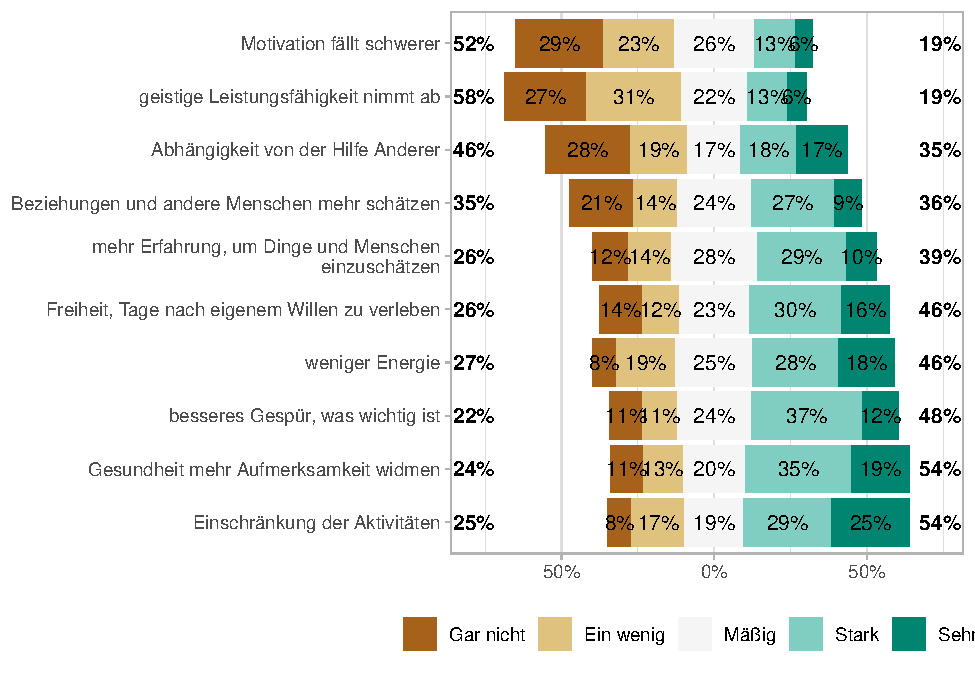
\includegraphics{desc_NRW80_files/figure-latex/likertalterl1-1.pdf}
\caption{\label{fig:likertalterl1}Experience of Ageing: Proportions of Answers (df\_alterl)}
\end{figure}

\begin{Shaded}
\begin{Highlighting}[]
\FunctionTok{gglikert}\NormalTok{(df\_alterl\_balance,}
         \AttributeTok{sort =} \StringTok{"ascending"}
\NormalTok{         )}
\end{Highlighting}
\end{Shaded}

\begin{figure}
\centering
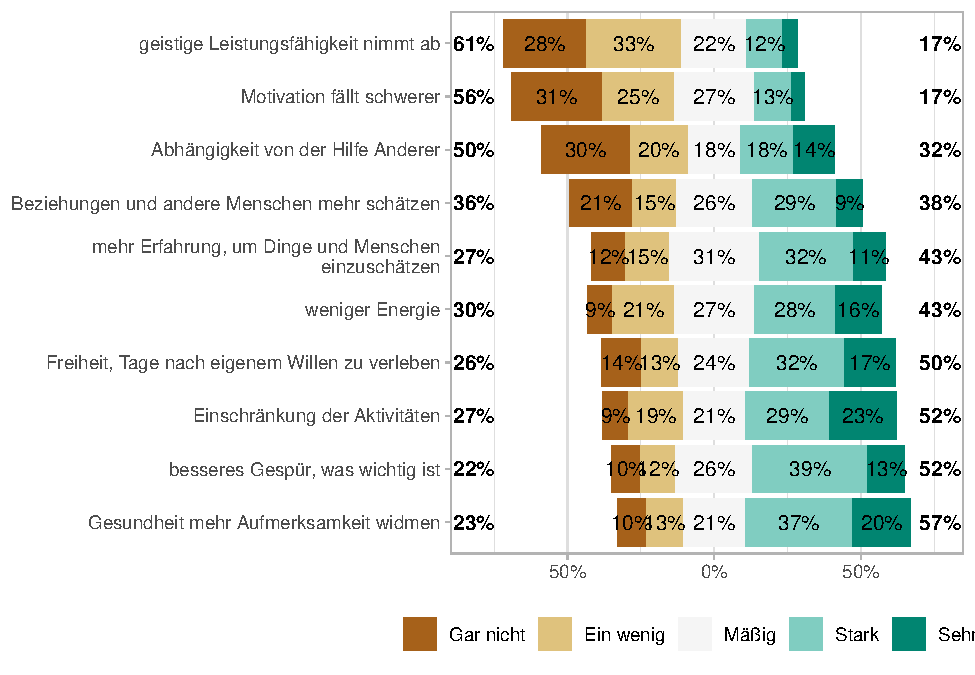
\includegraphics{desc_NRW80_files/figure-latex/likertalterl2-1.pdf}
\caption{\label{fig:likertalterl2}Experience of Ageing: Proportions of Answers (df\_alterl\_balance)}
\end{figure}

\begin{Shaded}
\begin{Highlighting}[]
\FunctionTok{gglikert\_stacked}\NormalTok{(df\_alterl,}
                 \AttributeTok{sort =} \StringTok{"ascending"}\NormalTok{,}
                 \AttributeTok{sort\_method =} \StringTok{"mean"}
\NormalTok{                 )}
\end{Highlighting}
\end{Shaded}

\begin{figure}
\centering
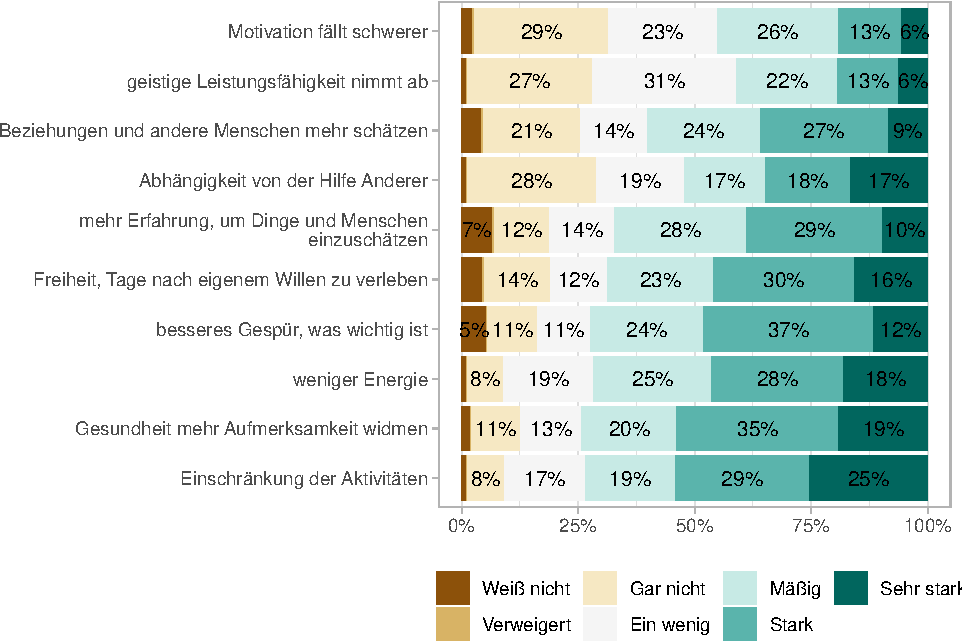
\includegraphics{desc_NRW80_files/figure-latex/likertalterl3-1.pdf}
\caption{\label{fig:likertalterl3}Experience of Ageing: Proportions of Answers - Stacked (df\_alter)}
\end{figure}

\begin{Shaded}
\begin{Highlighting}[]
\FunctionTok{gglikert\_stacked}\NormalTok{(df\_alterl\_balance,}
                 \AttributeTok{sort =} \StringTok{"ascending"}\NormalTok{,}
                 \AttributeTok{sort\_method =} \StringTok{"mean"}
\NormalTok{                 )}
\end{Highlighting}
\end{Shaded}

\begin{figure}
\centering
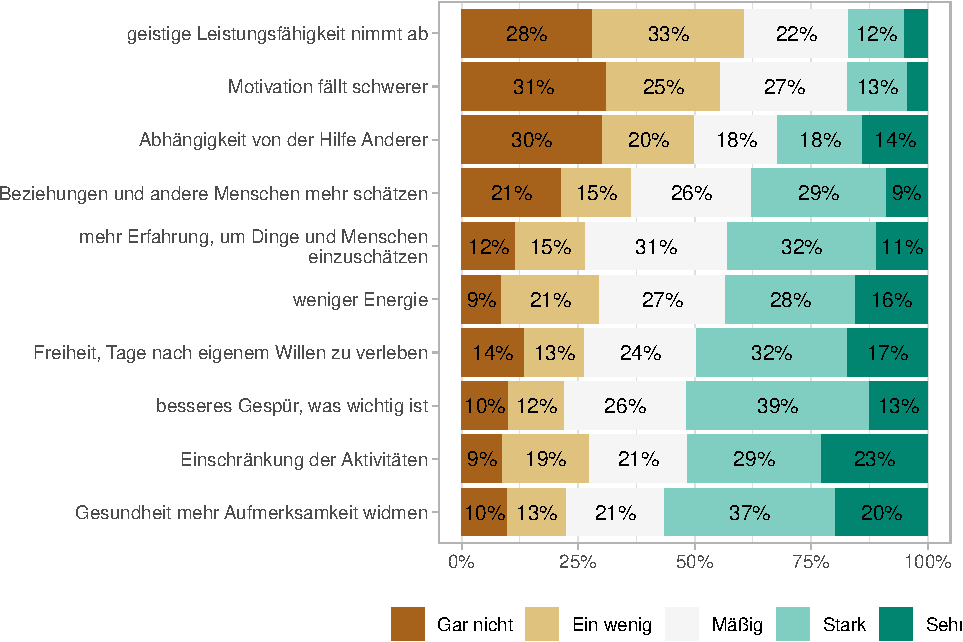
\includegraphics{desc_NRW80_files/figure-latex/likertalterl4-1.pdf}
\caption{\label{fig:likertalterl4}Experience of Ageing: Proportions of Answers - Stacked (df\_alterl\_balance)}
\end{figure}

As we are interested in the differences of the two samples, it makes sense to look as the summary statistics for the \texttt{df\_alter\_balance} sample. This is shown in Table \ref{tab:tabsumstatalterpsychbal}.

\begin{Shaded}
\begin{Highlighting}[]
\NormalTok{sumstat\_alter\_psych\_bal }\OtherTok{\textless{}{-}}\NormalTok{ df\_alterl\_balance }\SpecialCharTok{|\textgreater{}}
\NormalTok{  psych}\SpecialCharTok{::}\FunctionTok{describe}\NormalTok{() }\SpecialCharTok{|\textgreater{}} 
  \FunctionTok{as\_tibble}\NormalTok{(}\AttributeTok{rownames=}\StringTok{"Question"}\NormalTok{)  }\SpecialCharTok{|\textgreater{}} 
\NormalTok{  dplyr}\SpecialCharTok{::}\FunctionTok{select}\NormalTok{(}\SpecialCharTok{{-}}\NormalTok{skew, }\SpecialCharTok{{-}}\NormalTok{kurtosis, }\SpecialCharTok{{-}}\NormalTok{range, }\SpecialCharTok{{-}}\NormalTok{vars) }

\FunctionTok{apa\_table}\NormalTok{(}
\NormalTok{  sumstat\_alter\_psych\_bal}
\NormalTok{  , }\AttributeTok{caption =} \StringTok{"Summary Statistics: Experience of Ageing {-} balanced (psych)"}
\NormalTok{  , }\AttributeTok{note =} \StringTok{"This table contains all variables of \textasciigrave{}alterl*\textasciigrave{} and only observations where all questions had been answered."}
\NormalTok{  , }\AttributeTok{escape =} \ConstantTok{TRUE}
\NormalTok{)}
\end{Highlighting}
\end{Shaded}

\begin{table}[tbp]

\begin{center}
\begin{threeparttable}

\caption{\label{tab:tabsumstatalterpsychbal}Summary Statistics: Experience of Ageing - balanced (psych)}

\begin{tabular}{llllllllll}
\toprule
Question & \multicolumn{1}{c}{n} & \multicolumn{1}{c}{mean} & \multicolumn{1}{c}{sd} & \multicolumn{1}{c}{median} & \multicolumn{1}{c}{trimmed} & \multicolumn{1}{c}{mad} & \multicolumn{1}{c}{min} & \multicolumn{1}{c}{max} & \multicolumn{1}{c}{se}\\
\midrule
alterl1 & 1,596.00 & 2.89 & 1.28 & 3.00 & 2.87 & 1.48 & 1.00 & 5.00 & 0.03\\
alterl2 & 1,596.00 & 3.44 & 1.22 & 4.00 & 3.55 & 1.48 & 1.00 & 5.00 & 0.03\\
alterl3 & 1,596.00 & 2.33 & 1.15 & 2.00 & 2.23 & 1.48 & 1.00 & 5.00 & 0.03\\
alterl4 & 1,596.00 & 3.16 & 1.16 & 3.00 & 3.20 & 1.48 & 1.00 & 5.00 & 0.03\\
alterl5 & 1,596.00 & 3.32 & 1.15 & 4.00 & 3.40 & 1.48 & 1.00 & 5.00 & 0.03\\
alterl6 & 1,596.00 & 3.38 & 1.26 & 4.00 & 3.46 & 1.48 & 1.00 & 5.00 & 0.03\\
alterl7 & 1,596.00 & 3.21 & 1.19 & 3.00 & 3.24 & 1.48 & 1.00 & 5.00 & 0.03\\
alterl8 & 1,596.00 & 2.66 & 1.43 & 2.00 & 2.57 & 1.48 & 1.00 & 5.00 & 0.04\\
alterl9 & 1,596.00 & 3.27 & 1.27 & 3.00 & 3.34 & 1.48 & 1.00 & 5.00 & 0.03\\
alterl10 & 1,596.00 & 2.35 & 1.17 & 2.00 & 2.26 & 1.48 & 1.00 & 5.00 & 0.03\\
\bottomrule
\addlinespace
\end{tabular}

\begin{tablenotes}[para]
\normalsize{\textit{Anmerkungen.} This table contains all variables of `alterl*` and only observations where all questions had been answered.}
\end{tablenotes}

\end{threeparttable}
\end{center}

\end{table}

\clearpage

\hypertarget{cross-referencing-in-r-markdown}{%
\section{Cross-Referencing in R Markdown}\label{cross-referencing-in-r-markdown}}

In adherence to the APA style guidelines (Association et al., 2022), it is imperative to reference all figures and tables by their respective numbers within the text. Avoid using generic phrases like ``the table above'' or ``the figure below.'' Additionally, refrain from hard-coding the numbers for a more dynamic and standardized approach. Xie, Dervieux, and Riederer (2023) explains concisely how to do that with R Markdown, see: \url{https://bookdown.org/yihui/rmarkdown-cookbook/cross-ref.html}.

For example, I can refer to Table \ref{tab:tabrstatix} with \texttt{\textbackslash{}@ref(tab:tabrstatix)} because I have specified the corresponding label in the R code-chunk, see:

\begin{Shaded}
\begin{Highlighting}[]
\StringTok{\textasciigrave{}\textasciigrave{}\textasciigrave{}}\AttributeTok{\{r tabrstatix, echo=TRUE\}}
\AttributeTok{apa\_table(}
\AttributeTok{  sumstat\_alter}
\AttributeTok{  , caption = "Summary Statistics: Experience of Ageing."}
\AttributeTok{  , note = "This table contains all variables of }\StringTok{\textasciigrave{}}\NormalTok{alterl}\SpecialCharTok{*}\StringTok{\textasciigrave{}}\AttributeTok{."}
\AttributeTok{  , escape = TRUE}
\AttributeTok{  )}
\StringTok{\textasciigrave{}\textasciigrave{}\textasciigrave{}}
\end{Highlighting}
\end{Shaded}

\begin{verbatim}

\clearpage

# Exercises

1.  With `knitr::purl("desc_NRW80.Rmd")` you can extract the whole R code from the R Markdown file and write it into the R script `desc_NRW80.R`. Try it.

2.  The dataset `gesis.RData` comes with two different tibbles: `dfsav` and `dfdta`. Is there a difference between these two when it comes to the statistics that are shown in this paper? To check that, rename the pdf file `desc_NRW80.pdf`, change the code in Section \\ref{sec-load} so that you are using the other data (`df <- dfdta |> ...` vs. `df <- dfsav |> ...`), knit the Rmd again, and compare the stats.

3.  Check possible differences in the `gglikert` plots when using `df_alterl_un` instead of `df_alterl`.

4.  The stats above show that dealing with missing or non-standard answers is a crucial thing. Please read chapter *Missing Values* of @Wickham2023R, see: <https://r4ds.hadley.nz/missing-values>.

5. The labels of the variables `alterl1:alterl10` have "Alternserleben: " at the beginning. This is not necessary and overloads the graphs. Please change the labels for all graphs using the following code in the respective place in the rmd and then knit it again.



```r
# Remove the common prefix from all variables
df <- df |> 
  mutate_all(~ set_label(., gsub("^Alternserleben: ", "", get_label(.))))
\end{verbatim}

\clearpage

\hypertarget{references}{%
\section*{References}\label{references}}
\addcontentsline{toc}{section}{References}

\hypertarget{refs}{}
\begin{CSLReferences}{1}{0}
\leavevmode\vadjust pre{\hypertarget{ref-Association2022Publication}{}}%
Association, A. P. et al. (2022). \emph{Publication manual of the american psychological association}. : American Psychological Association.

\leavevmode\vadjust pre{\hypertarget{ref-Aust2020papaja}{}}%
Aust, F., \& Barth, M. (2020). \emph{Papaja: Reproducible APA manuscripts with r markdown}. Retrieved from \url{https://frederikaust.com/papaja_man/}

\leavevmode\vadjust pre{\hypertarget{ref-R-papaja}{}}%
Aust, F., \& Barth, M. (2023). \emph{{papaja}: {Prepare} reproducible {APA} journal articles with {R Markdown}}. Retrieved from \url{https://github.com/crsh/papaja}

\leavevmode\vadjust pre{\hypertarget{ref-Firke2023janitor}{}}%
Firke, S. (2023). \emph{Janitor: Simple tools for examining and cleaning dirty data}. Retrieved from \url{https://CRAN.R-project.org/package=janitor}

\leavevmode\vadjust pre{\hypertarget{ref-Kassambara2023rstatix}{}}%
Kassambara, A. (2023). \emph{Rstatix: Pipe-friendly framework for basic statistical tests}. Retrieved from \url{https://CRAN.R-project.org/package=rstatix}

\leavevmode\vadjust pre{\hypertarget{ref-Larmarange2023ggstats}{}}%
Larmarange, J. (2023). \emph{Ggstats: Extension to 'ggplot2' for plotting stats}. Retrieved from \url{https://CRAN.R-project.org/package=ggstats}

\leavevmode\vadjust pre{\hypertarget{ref-Luedecke2018sjmisc}{}}%
Lüdecke, D. (2018). Sjmisc: Data and variable transformation functions. \emph{Journal of Open Source Software}, \emph{3}(26), 754. \url{https://doi.org/10.21105/joss.00754}

\leavevmode\vadjust pre{\hypertarget{ref-Wickham2023dplyr}{}}%
Wickham, H., François, R., Henry, L., Müller, K., \& Vaughan, D. (2023). \emph{Dplyr: A grammar of data manipulation}. Retrieved from \url{https://CRAN.R-project.org/package=dplyr}

\leavevmode\vadjust pre{\hypertarget{ref-Wickham2023purrr}{}}%
Wickham, H., \& Henry, L. (2023). \emph{Purrr: Functional programming tools}. Retrieved from \url{https://CRAN.R-project.org/package=purrr}

\leavevmode\vadjust pre{\hypertarget{ref-WilliamRevelle2023psych}{}}%
William Revelle. (2023). \emph{Psych: Procedures for psychological, psychometric, and personality research}. Evanston, Illinois: Northwestern University. Retrieved from \url{https://CRAN.R-project.org/package=psych}

\leavevmode\vadjust pre{\hypertarget{ref-Xie2023R}{}}%
Xie, Y., Dervieux, C., \& Riederer, E. (2023). \emph{R markdown cookbook}. online. Retrieved from \url{https://bookdown.org/yihui/rmarkdown-cookbook/}

\leavevmode\vadjust pre{\hypertarget{ref-Zank2022Quality}{}}%
Zank, S., Woopen, C., Wagner, M., Rietz, C., \& Kaspar, R. (2022). \emph{Quality of life and well-being of very old people in NRW (representative survey NRW80+) - cross-section wave 1}. GESIS, Cologne. ZA7558 Data file Version 2.0.0. \url{https://doi.org/10.4232/1.13978}

\end{CSLReferences}


\clearpage
\renewcommand{\listfigurename}{Figure captions}

\clearpage
\renewcommand{\listtablename}{Table captions}


\end{document}
